\documentclass[12pt]{article}
\usepackage[shortlabels]{enumitem}
\usepackage{placeins}
\usepackage{graphicx}
\begin{document}
\title{TCES 420 - Week 8}
\author{Jake McKenzie}
\maketitle
\noindent\centerline{\textbf{Homework 7}}
\textbf{Section 1}
9.18 A certain computer provides its users with a virtual memory space of
$2^{32}$ bytes. The computer has $2^{22}$ bytes of physical memory. The virtual
memory is implemented by paging, and the page size is $4,096$ bytes.
A user process generates the virtual address $11123456$. Explain how
the system establishes the corresponding physical location. Distinguish
between software and hardware operations.\\\\
\textbf{Answer: } If we convert the virtual address from decimal to 
hex we obtain $11123456_{10}$ $=$ $0$x$00$A$9$BB$00$. We can obtain the 
page size of $2^(12)$ thus the first $12$ bits are for displacement within pages 
and we can deduce that the displacement within the table is $20$ bits 
because the table size is $2^(20)$. We obtain a $0$x$00$A$9$B for the pages 
table displacement and $0$xB$00$ for pages displacement.\\\\
9.19 Assume that we have a demand-paged memory. The page table is held in
registers. It takes 8 milliseconds to service a page fault if an empty frame
is available or if the replaced page is not modified and $20$ milliseconds if
the replaced page is modified. Memory-access time is $100$ nanoseconds.
Assume that the page to be replaced is modified $70$ percent of the
time. What is the maximum acceptable page-fault rate for an effective
access time of no more than $200$ nanoseconds?\\\\
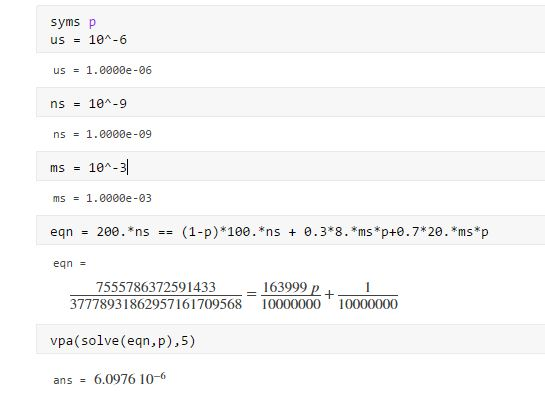
\includegraphics[scale = 1]{q19.JPG}\\
\textbf{Answer: } $p = 6.0976*10^{-6}$\\
When a page fault occurs, the process requesting the page must block
while waiting for the page to be brought from disk into physical memory.
Assume that there exists a process with five user-level threads and that
the mapping of user threads to kernel threads is one to one. If one user
thread incurs a page fault while accessing its stack, would the other
user threads belonging to the same process also be affected by the page
fault—that is, would they also have to wait for the faulting page to be
brought into memory? Explain.\\\\
\textbf{Answer: }If you have multiple threads, while one thread is blocking which is the case
in this example, the other threads in this process will be uneffected by 
the blocking.  Only on that single thread who is blocking is there an 
negative effect from the page fault.\\\\
9.22 The page table shown in Figure $9.32$ is for a system with 16-bit virtual
and physical addresses and with $4,096$-byte pages. The reference bit is
set to $1$ when the page has been referenced. Periodically, a thread zeroes
out all values of the reference bit. A dash for a page frame indicates
the page is not in memory. The page-replacement algorithm is localized
LRU, and all numbers are provided in decimal.\\\\
a) Convert the following virtual addresses (in hexadecimal) to the
equivalent physical addresses. You may provide answers in either 
hexadecimal or decimal. Also set the reference bit for the appropriate
entry in the page table.\\\\
\textbf{Answer: }\\
Virtual Address $\sim$ physical address\\
$0$xE$12$C $\sim$ $0$x$312$C\\
$0$x$3$A$9$D $\sim$ $0$xAA$9$D\\
$0$xA$9$D$9$ $\sim$ $0$x$59$D$9$\\
$0$x$7001$ $\sim$ $0$xF$001$\\
$0$xACA$1$ $\sim$ $0$x$5$CA$1$
\\\\
b) Using the above addresses as a guide, provide an example of a
logical address (in hexadecimal) that results in a page fault.\\\\
\textbf{Answer: } $0$x$4$, $0$x$8$, $0$xC and $0$xD are all page 
frames that will result in page faults
\\\\
c) From what set of page frames will the LRU page-replacement
algorithm choose in resolving a page fault?\\\\
\textbf{Answer: } I don't know how to do this and I'm completely lost.
You also won't even look at this so what even is the point.\\\\
9.23 Assume that you are monitoring the rate at which the pointer in the
clock algorithm moves. (The pointer indicates the candidate page for
replacement.) What can you say about the system if you notice the
following behavior:\\
a) pointer is moving fast.\\
\textbf{Answer: } If the pointer is moving quickly that would imply there 
are very few page faults and that we are accessing a lot of pages.
\\\\
b) pointer is moving slow.\\
\textbf{Answer: } If the power is moving slowly that would imply there are 
very many page faults and that we are not accessing many pages.
\\\\
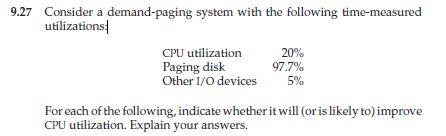
\includegraphics[scale = 1]{q27.JPG}\\\
a. Install a faster CPU.\\\\
\textbf{Answer: } A faster CPU, in theory, should reduce its utilization by 
accomplishing more tasks more quickly.
\\\\
b. Install a bigger paging disk.\\\\
\textbf{Answer: } Having more room for pages will not do anything to CPU usuage.
\\\\
c. Increase the degree of multiprogramming.\\\\
\textbf{Answer: } This will make the CPU utilization worse because the number of 
page faults will increase as the degree of multiprogramming increases.
\\\\
d. Decrease the degree of multiprogramming.\\\\
\textbf{Answer: }This will make the CPU utilization better because the number of 
page faults will decrease as the degree of multiprogramming decreases.
\\\\
e. Install more main memory.\\\\
\textbf{Answer: } More main memory means more room for active pages meaning less 
page faults, leading to less CPU utilization.
\\\\
f. Install a faster hard disk or multiple controllers with multiple hard
disks.\\\\
\textbf{Answer: } This will increase the overall throughput of the system, but 
the overall utilization statistics should stay constant.
\\\\
g. Add prepaging to the page-fetch algorithms.\\\\
\textbf{Answer: } This will increase cpu utilization as the cpu has to do more 
work for each paging request.
\\\\
h. Increase the page size.\\\\
\textbf{Answer: } Increasing the size of each page will decrease the amount of overall 
pages which means there are less pages to fault, reducing cpu utilization.
\\\\
9.30 A page-replacement algorithm should minimize the number of page
faults. We can achieve this minimization by distributing heavily used
pages evenly over all of memory, rather than having them compete for
a small number of page frames. We can associate with each page frame
a counter of the number of pages associated with that frame. Then,
to replace a page, we can search for the page frame with the smallest
counter.\\\\
a) Define a page-replacement algorithm using this basic idea. Specifically
address these problems:\\
i. What is the initial value of the counters?\\
\textbf{Answer: } counter $=$ $0$
\\
ii. When are counters increased?\\
\textbf{Answer: }Whenever a new page is associated with a frame in current 
context the counter is increased.
\\
iii. When are counters decreased?\\
\textbf{Answer: }Whenever a new page is associated with a frame that is not 
in current context the counter is increased.
\\
iv. How is the page to be replaced selected?\\
\textbf{Answer: } Whichever page exists in a frame that has the smaller 
counter where ties are broken by whoever arrives first (FIFO).
\\
b) How many page faults occur for your algorithm for the followingn
reference string with four page frames?\\
\centerline{$1, 2, 3, 4, 5, 3, 4, 1, 6, 7, 8, 7, 8, 9, 7, 8, 9, 5, 4, 5, 4, 2$}\\
\textbf{Answer: }\\
\centerline{F,F,F,F,F,F,-,F,F,F,F,-,-,F,-,-,-,F,F,-,-,F}\\
I found there were $14$ page faults.
\\
c) What is the minimum number of page faults for an optimal pagereplacement
strategy for the reference string in part b with four
page frames?\\
\centerline{$1, 2, 3, 4, 5, 3, 4, 1, 6, 7, 8, 7, 8, 9, 7, 8, 9, 5, 4, 5, 4, 2$}\\
\textbf{Answer: }\\\\
\centerline{F,F,F,F,F,-,-,-,F,F,F,-,-,F,-,-,-,-,F,F}\\
If found there were $11$ page faults.
\\\\
9.32 What is the cause of thrashing? How does the system detect thrashing?
Once it detects thrashing, what can the system do to eliminate this
problem?\\
\textbf{Answer: }\\
Thrashing occurs when a computer's virtual memory resources are overused, 
leading to a constant state of paging and page faults, inhibiting most 
application-level processing. By tracking working sets, we can detect 
thrashing by comparing the total working set size to the number of frames 
of available memory. We can also make use of the size of the working sets 
when determining which processes to suspend.\\\\
\textbf{Section 2}\\
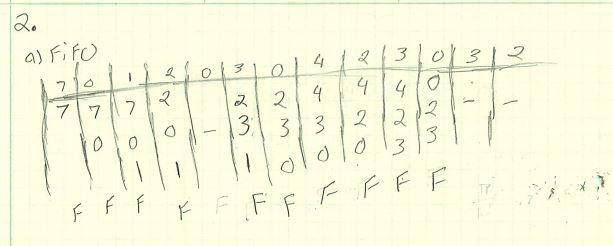
\includegraphics[scale = 1]{2a.JPG}\\
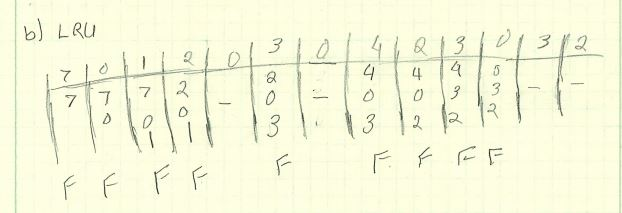
\includegraphics[scale = 1]{2b.JPG}\\
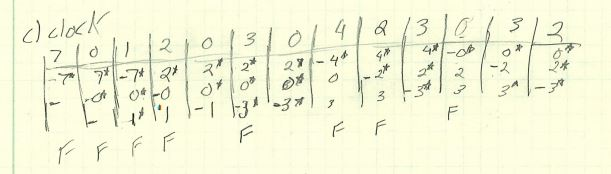
\includegraphics[scale = 1]{2c.JPG}\\
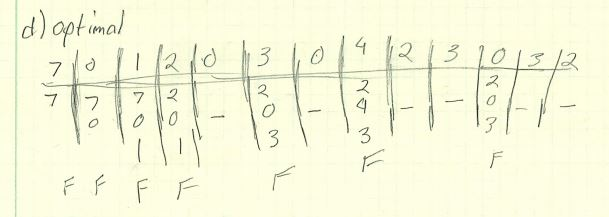
\includegraphics[scale = 1]{2d.JPG}\\
2. e) \\
For 2. a) I found there were $7$ total page faults with miss rate 
of $70\%$ and for 2. b) I found there were $6$ total page faults with miss rate 
of $60\%$ and for 2. c) I found there were $5$ total page faults with miss rate 
of $50\%$ and for 2. d) I found there were $4$ total page faults with miss rate 
of $40\%$. \\\\
\textbf{Section 3}\\
a) There are $2^5$ total pages that take up $2$ KBytes each. That gives us 
logical page number of $5$ and an offset of $11$ because $2$ KBytes $=$ $2^1*2^{10}$ 
$=$ $2^{11}$ .\\\\
b) The width $=$ $\frac{1MB}{2Kb}$ $=$ $\frac{2^{20}}{2^11}$ $=$ $2^9$ so the width is 
$9$ bits. There are $32$ pages so there must be a length of $32$ to account for each 
page.\\\\
c) Making physical memory space reduce by half means shifting to the left 
by $1$ or to show my work $\frac{2^19}{2^11} = 2^8$. Now the width is effectively 
$8$ bits.\\
\textbf{Section 4}\\
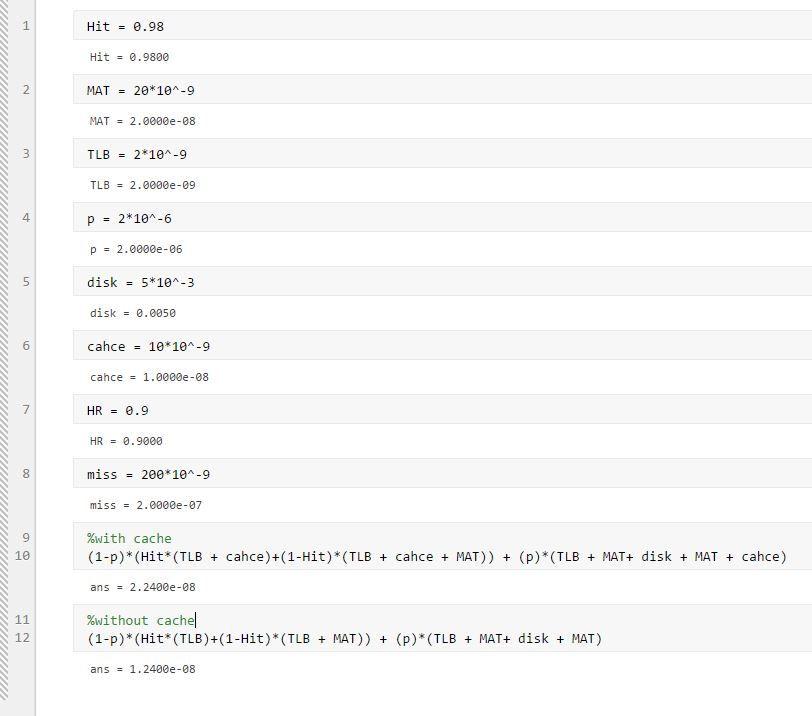
\includegraphics[scale = 1]{4.JPG}\\
With a cache I got an Overall EAT $=$ $22.4$ns and without cache an Overall EAT $=$ $12.4$ns.
\\\\
\textbf{Section 5}\\
\end{document}